\documentclass[12pt]{article}

% Put your name/s and ID number/s here
\newcommand{\myname}{Your Full Name Here}
\newcommand{\myidnumber}{220000}
 \newcommand{\mysection}{X}
 
% Put the problem set number here
\newcommand{\psetnumber}{Y}

\usepackage{probset}

\begin{document}
\problem{1}
You can write pseudocode in a similar style as the course notes using the \verb|algorithmic| environment.

Here are some sample pseudocode.
\begin{algorithmic}[1]
\Proc{ListMax}{$L$}
    \State $\Id{max} \gets L[1]$
    \Comment{this is the first element of $L$}
    \For{$i \gets 2 \To \attrib{L}{length}$}
        \If{$L[i] > \Id{max}$}
            \State $\Id{max} \gets L[i]$
        \EndIf
    \EndFor
    \Return \Id{max}
\end{algorithmic}

The assignment operator ($\gets$) is typeset using \verb|\gets|, while the equality operator ($\isequal$) is typeset using \verb|\isequal|. Don't use the plain \verb|=| character!

\textbf{Important!} If typesetting variables with two or more characters, use \verb|\Id{abcdefghijk}| instead of \verb|$abcdefghijk$| so the spacing between letters isn't wack: $\Id{abcdefghijk}$ vs. $abcdefghijk$.
\begin{algorithmic}[1]
\Proc{FormSubsets}{\Id{elems}, \Id{chosen}}
    \If{\Id{elems} is empty}
    \Comment{no decisions remain}
        \State print \Id{chosen}
    \Else
    \Comment{try all options for the next decision}
        \State $e \gets \Call{Pick}{\Id{elems}}$
        \Comment{pick an element from the set}
        \State $\Id{remaining} \gets \Id{elems} \setminus \Set{e}$
        \Comment{remove this element from possible choices}
        \State \Call{FormSubsets}{\Id{remaining}, $\Id{chosen} \cup \Set{e}$}
        \Comment{either include this element}
        \State \Call{FormSubsets}{\Id{remaining}, \Id{chosen}}
        \Comment{or exclude this element}
    \EndIf
\end{algorithmic}

Here's another example with the while loop:
\begin{algorithmic}[1]
\Proc{HeapIncreaseKey}{$A$, $i$, \Id{key}}
    \If{$\Id{key} < A[i]$}
        \State error ``new key is smaller than current key''
    \EndIf
    \State $A[i] \gets \Id{key}$
    \While{$i > 1$ and $A[\Call{Parent}{i}] < A[i]$}
        \State swap $A[i]$ with $A[\Call{Parent}{i}]$
        \State $i \gets \Call{Parent}{i}$
    \EndWhile
\end{algorithmic}

Attributes of an object are typeset as \verb|\attrib{X}{attr}| or \verb|\attrib{\Id{obj}}{attr}|: \attrib{X}{attr} or \attrib{\Id{obj}}{attr}.
\textbf{More advanced stuff:} If you want two algorithms side-by-side, use the \verb|minipage| environment:
\begin{center}
    \begin{minipage}{0.45\textwidth}
    \begin{algorithmic}[1]
    \Proc{MergeSort}{$A$}
        \If{$\attrib{A}{length} \isequal 1$}
            \Return $A$
        \EndIf
        \State $m \gets \lfloor \attrib{A}{length}/2 \rfloor$
        \State $L \gets \text{\Call{MergeSort}{$A[\subarr m]$}}$
        \State $R \gets \text{\Call{MergeSort}{$A[m+1\subarr]$}}$
        \State $S \gets \text{\Call{Merge}{$L$, $R$}}$
        \Return $S$
    \end{algorithmic}
    \end{minipage}
    \begin{minipage}{0.5\textwidth}
    \begin{algorithmic}[1]
    \Proc{Merge}{$L$, $R$}
        \State let $A[1\subarr n]$ be an empty array
        \State $i \gets 1$, $j \gets 1$
        \For{$k \gets 1 \To n$}
            \If{$L[i] \le R[j]$}
                \State $A[k] \gets L[i]$;\quad$i \gets i+1$
            \Else
                \State $A[k] \gets R[j]$;\quad$j \gets j+1$
            \EndIf
        \EndFor
        \Return $A$
    \end{algorithmic}
    \end{minipage}
\end{center}

\problem{2}
Here are my sample answers to essay questions using the \verb|enumerate| environment:
\begin{enumerate}
    \item Hell no! There's no way an incorrect algorithm is useful. Why bother? Ugh\ldots
    
    \item I got scared of this question. As such, the answer is skipped.
    
    \item The problem with benchmarking is that not all computers are created equally; just the hardware within it will certainly differ from one computer to another. Some programs might run quickly on one computer, but very slowly in another. You need to have the same machine setup every time you compare algorithms.
    
    \item Nah, I'm not gonna answer this. Skipped!
    
\end{enumerate}

For unordered/bulleted lists, you can use the \verb|itemize| environment instead.

\problem{3}
Here's a sample usage of the \texttt{theorem} and \texttt{proof} environments.

\begin{theorem*}
A context-free grammar is said to be right-linear if all productions are of the form $A \rightarrow wB$ or $A \rightarrow w$, where $A$ and $B$ are variables and $w$ is a string of zero or more terminals. Then every right-linear grammar generates a regular language.
\end{theorem*}
\begin{proof}
The proof is exercising social distancing. As such, its fine details cannot be revealed until the pandemic is over. What I do know is the Citardauq formula:
\[
    x = \frac{2c}{-b \mp \sqrt{b^2 - 4ac}}.
\]
I hope this completes the proof.
\end{proof}

Here's an example of a numbered theorem.
% numbered theorem
\begin{theorem}[Add optional description here]
    The one-time pad is perfectly secret.
\end{theorem}
\begin{proof}
    We first compute $\Pr[C = c \mid M = m]$ for arbitrary $c \in \mathcal{C}$ and $m \in \mathcal{M}$ with $\Pr[M = m] > 0$. For the one-time pad, we have
    \begin{align*}
        \Pr[C = c \mid M = m] &= \Pr[K \oplus m = c \mid M = m] & \text{(by definition)} \\
        &= \Pr[K = m \oplus c \mid M = m] \\
        &= 2^{-n}.
    \end{align*}
    where the final equality holds because $K$ is a uniform $n$-bit string independent of $M$. 
    Fix any distribution over $\mathcal{M}$. Then for any $c \in \mathcal{C}$, we have
    \begin{align*}
        \Pr[C = c] &= \sum_{m \in \mathcal{M}} \Pr[C = c \mid M = m] \cdot \Pr[M = m] & \text{(law of total probability)} \\
        &= 2^{-n} \cdot \sum_{m \in \mathcal{M}} \Pr[M = m] & \text{(from above result)} \\
        &= 2^{-n} & \text{(second axiom of probability)}
    \end{align*}
    where $\Pr[M = m] \ne 0$.
    Bayes' theorem gives us:
    \begin{align*}
        \Pr[M = m \mid C = c] &= \frac{\Pr[C = c \mid M = m] \cdot \Pr[M = m]}{\Pr[C = c]} \\
        &= \frac{2^{-n} \cdot \Pr[M = m]}{2^{-n}} \\
        &= \Pr[M = m].
    \end{align*}
    Therefore the one-time pad is perfectly secret.
\end{proof}

\problem{4}
Here's a picture that hopefully explains my solution to this problem:
\begin{figure}[H]
    \centering
    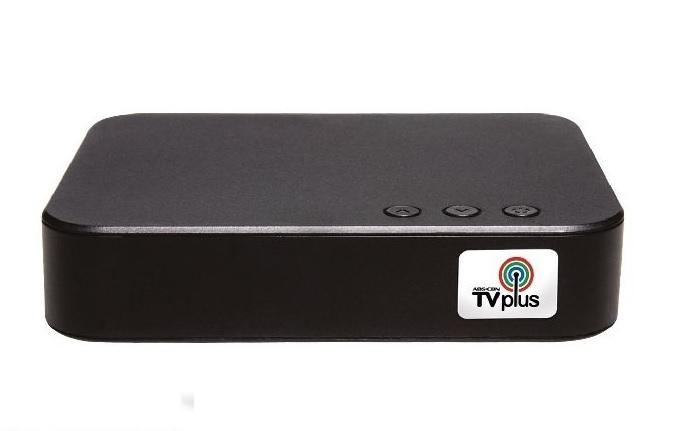
\includegraphics[width=7cm]{blackbox.jpg}
    \caption{An algorithm is a magical black box that does magical computer things.}
\end{figure}

\problem{5}
Here is a snippet of Python code:
\begin{minted}{python}
class LinkedList(object):
    def __init__(self, head=None):
        self.head = head
    def __repr__(self):
        node = self.head
        lst = []
        if node is not None:
            while node.get_next() is not None:
                lst += [node.get_item()]
                node = node.get_next()
            if node is not None:
                lst += [node.get_item()]
        return f'Linked list of {len(lst)} elements consisting of {str(lst)}'
    
    def insert(self, e):
        new_node = Node(e)
        new_node.set_next(self.head)
        self.head = new_node
        
    def search(self, e):
        x = self.head
        while x is not None and x.get_item() != e:
            x = x.get_next()
        return x
        
    def delete(self, e):
        # search for the node containing the item to be deleted
        x, prev = self.head, None
        
        # if the head node contains that element
        if x is not None and x.get_item() == e:
            self.head = x.get_next()
        else:
            while x is not None and x.get_item() != e:
                prev = x
                x = x.get_next()
            # then unlink the node from linked list
            if x is not None:
                prev.set_next(x.get_next())

\end{minted}

Here is a snippet of C++ code:
\begin{minted}{c++}
#include <bits/stdc++.h>

using namespace std;
typedef long long ll;

const double EPS = 1e-7;
double A[30][30];

bool rref(int n, int m) {
    bool singular = false;
    for (int i=0, p=0; i < n && p < m; i++, p++) {
        for (int k = i+1; k < n; k++) {
            if (abs(A[k][p]) > EPS) {
                for (int l = 0; l < m; l++) {
                    double t = A[i][l];
                    A[i][l] = A[k][l];
                    A[k][l] = t;
                }
                break;
            }
        }
        if (abs(A[i][p]) < EPS) {
            singular = true; i--;
            continue;
        }
        for (int j = m-1; j >= p; j--)
            A[i][j] /= A[i][p];
        for (int k = 0; k < n; k++) {
            if (i == k) continue;
            for (int j = m-1; j >= p; j--)
                A[k][j] -= A[k][p] * A[i][j];
        }
    }
    return !singular;
}
\end{minted}

\problem{6}
% helpful macros for problem 1-2
\newcommand{\lb}{\textbf{\s{[}}}
\newcommand{\rb}{\s{]}}
\newcommand{\aeplus}{\,\s{+}\,}
\newcommand{\aetimes}{\,\s{*}\,}
\newcommand{\aeAdd}[2]{\lb #1 \aeplus #2 \rb}
\newcommand{\aeMul}[2]{\lb #1 \aetimes #2 \rb}
\newcommand{\aeNeg}[1]{\s{-}\, \lb #1 \rb}

For example, here's how the recursive definition of eval would arrive at the value of $3 + x^2$ when $x$ is $2$:
\begin{align*}
    \eval(\aeAdd{\s{3}}{\aeMul{x}{x}}, 2) &= \eval(\s{3}, 2) + \eval(\aeMul{x}{x}, 2) & \text{(by rule~3)} \\
    &= 3 + \eval(\aeMul{x}{x}, 2) & \text{(by rule~2)} \\
    &= 3 + (\eval(x, 2) \cdot \eval(x, 2)) & \text{(by rule~4)} \\
    &= 3 + (2 \cdot 2) & \text{(by rule~1)} \\
    &= 3 + 4 = 7.
\end{align*}

Here's how the recursive definition of the substitution function would find the result of substituting $3x$ for $x$ in the expression $x(x-1)$:
\begin{align*}
    &\subst(3x, x(x-1)) \\
    &= \subst(\aeMul{\s{3}}{x}, \aeMul{x}{\aeAdd{x}{\aeNeg{\s{1}}}}) & \text{(unabbreviating)} \\
    &= \aeMul{\subst(\aeMul{\s{3}}{x}, x)}{\subst(\aeMul{\s{3}}{x}, \aeAdd{x}{\aeNeg{\s{1}}})} & \text{(by rule~9)} \\
    &= \aeMul{\aeMul{\s{3}}{x}}{\subst(\aeMul{\s{3}}{x}, \aeAdd{x}{\aeNeg{\s{1}}})} & \text{(by rule~6)} \\
    &= \aeMul{\aeMul{\s{3}}{x}}{\aeAdd{\subst(\aeMul{\s{3}}{x},     x)}{\subst(\aeMul{\s{3}}{x}, \aeNeg{\s{1}})}} & \text{(by rule~8)} \\
    &= \aeMul{\aeMul{\s{3}}{x}}{\aeAdd{\aeMul{\s{3}}{x}}{\subst(\aeMul{\s{3}}{x}, \aeNeg{\s{1}})}} & \text{(by rule~6)} \\
    &= \aeMul{\aeMul{\s{3}}{x}}{\aeAdd{\aeMul{\s{3}}{x}}{\aeNeg{\subst(\aeMul{\s{3}}{x}, \s{1}})}} & \text{(by rule~10)} \\
    &= \aeMul{\aeMul{\s{3}}{x}}{\aeAdd{\aeMul{\s{3}}{x}}{\aeNeg{\s{1}}}} & \text{(by rule~7)} \\
    &= 3x(3x-1) & \text{(abbreviation)}
\end{align*}

Also, sus:
\begin{figure}[H]
    \centering
    \begin{tikzpicture}[every path/.style={very thick}]
        \amongUsI{cyan}{cyan!30}
        \amongUsHandsB[shift={(0,3)}]{cyan}
        \amongUsHandsB[xscale=-1, shift={(-4,3)}]{cyan}
    \end{tikzpicture}
\end{figure}

\end{document}
